\section{Introduction}
\label{ch:intro}

The Coronavirus disease (COVID-19) was first characterized by the World Health Organisation as pandemic on 11th March 2020 \cite{whodeclare20}. The outbreak has affected almost every aspect of human life throughout 2020, and is expected to continue for much of 2021. 

\begin{figure}[H]
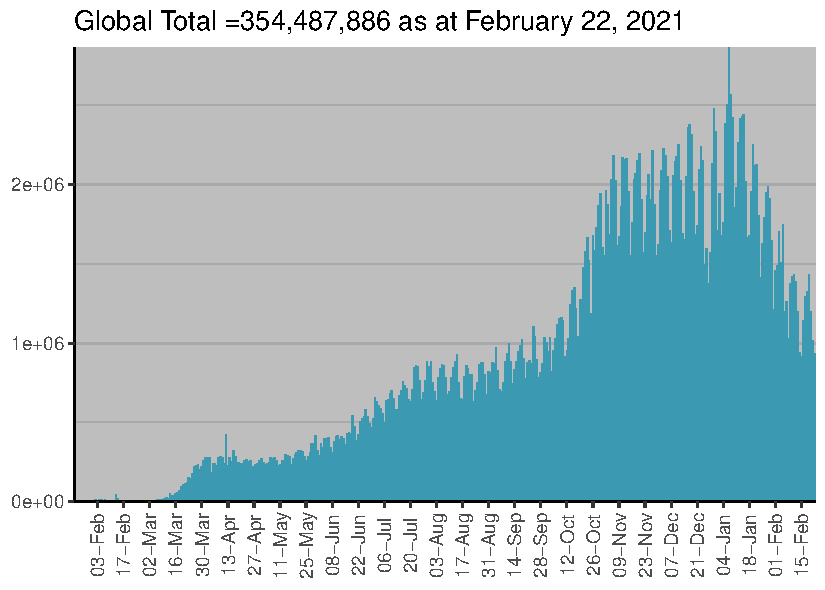
\includegraphics[width=0.9\textwidth]{WorldTotal-xn.pdf}
\caption{Daily Cases Globally}
\end{figure}

We can map the cumulative number of cases per 100,000 population for each country to see the varying severity of disease spread. 

\begin{figure}[H]
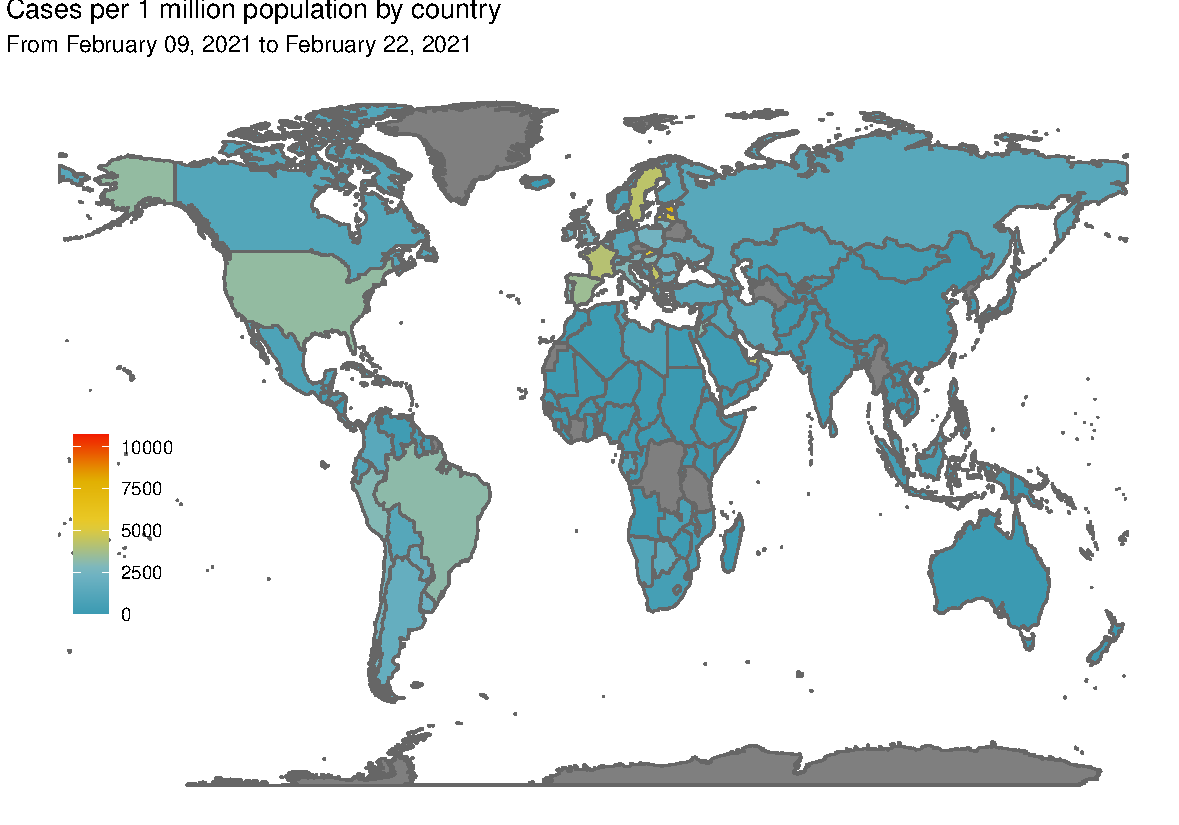
\includegraphics[width=0.9\textwidth]{world-blank.pdf}
\caption{Cases per 1 million population, World}
\end{figure}

Europe is experiencing an especially high number of cases, proportionally, as well as the US.

\begin{figure}[H]
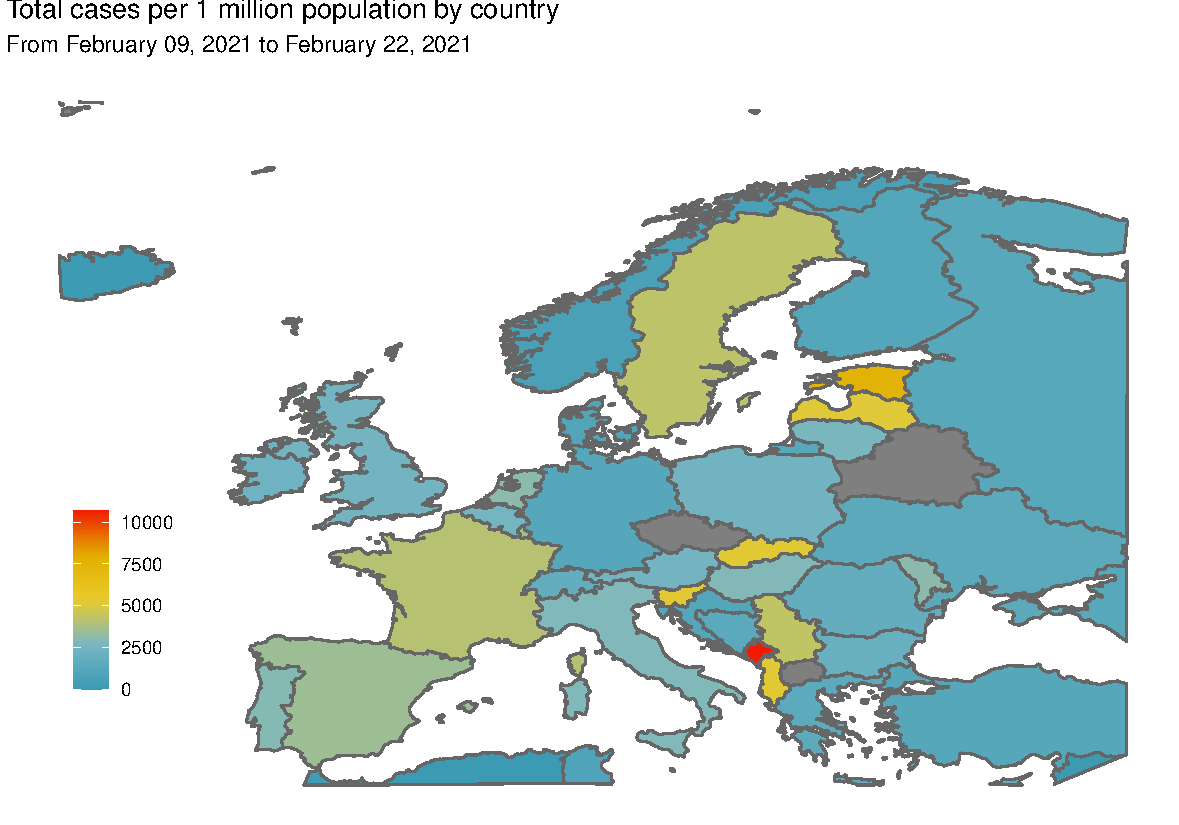
\includegraphics[width=0.9\textwidth]{world-europe.pdf}
\caption{Cases per 1 million population,  Europe}
\end{figure}

More locally, we see that Ireland also has a clear variation in concentration of cases to date, with Donegal and much of Leinster experiencing sometimes twice as many cases per 100,000 population as the rest of the country.

\begin{figure}[H]
\minipage{0.48\textwidth}
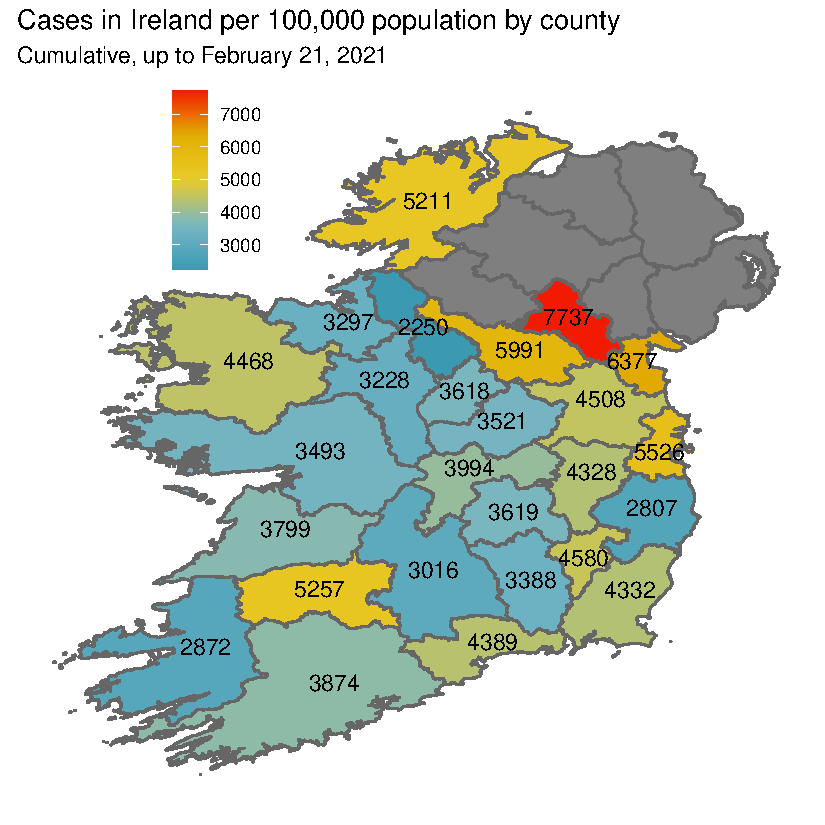
\includegraphics[width=0.9\textwidth]{county-rep.pdf}
\endminipage\hfill
\minipage{0.48\textwidth}
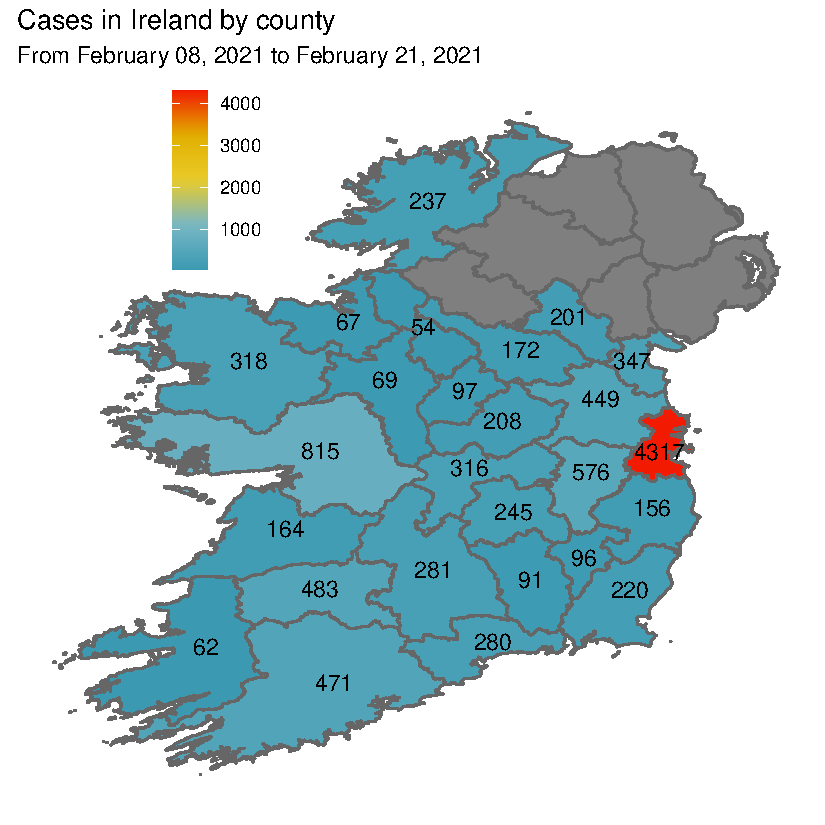
\includegraphics[width=0.9\textwidth]{county-fourteendaycases.pdf}
\endminipage
\caption{Situation by County, Ireland}
\end{figure}

\begin{figure}[H]
\minipage{0.48\textwidth}
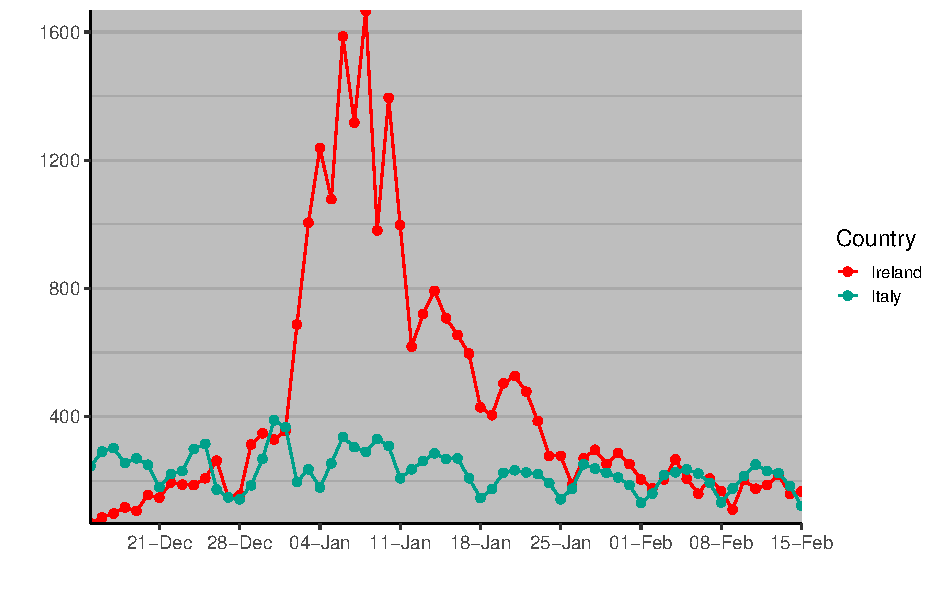
\includegraphics[width=0.9\textwidth]{compare-IreIta.pdf}
\endminipage\hfill
\minipage{0.48\textwidth}
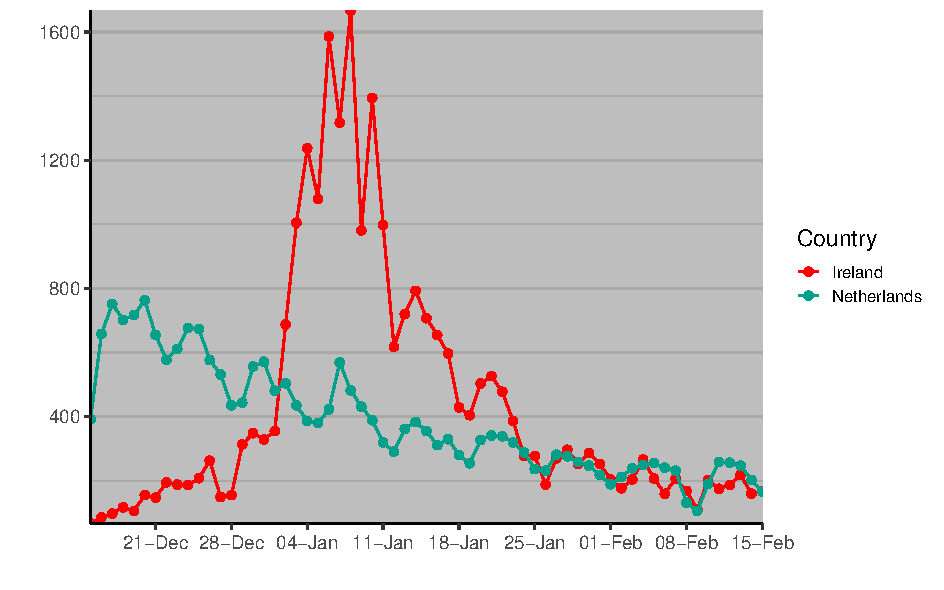
\includegraphics[width=0.9\textwidth]{compare-IreNl.pdf}
\endminipage \\
\minipage{0.48\textwidth}
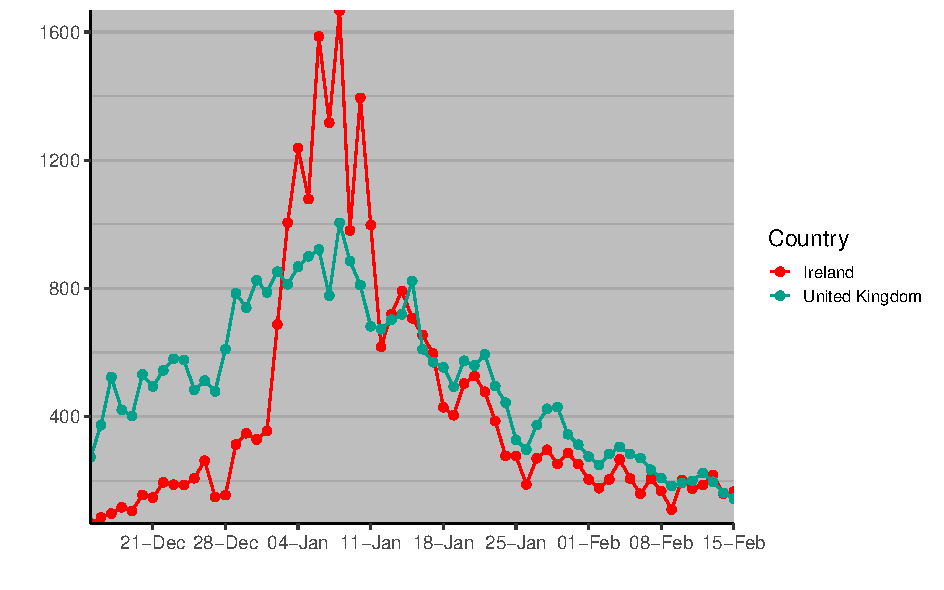
\includegraphics[width=0.9\textwidth]{compare-IreUK.pdf}
\endminipage\hfill
\minipage{0.48\textwidth}
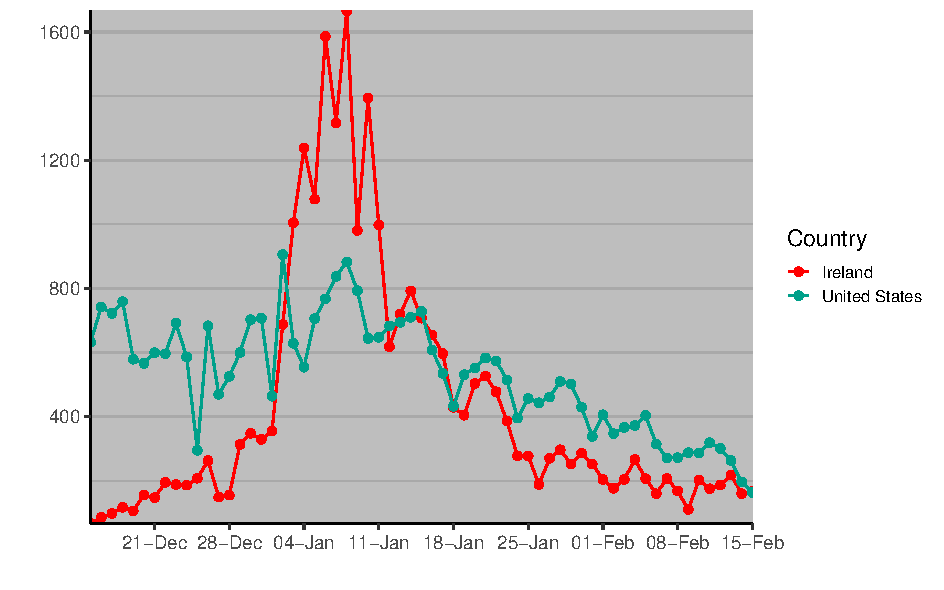
\includegraphics[width=0.9\textwidth]{compare-IreUS.pdf}
\endminipage
\caption{Individual Comparison of Ireland with various countries, daily cases per million of the population}
\end{figure}

\begin{figure}[H]
\minipage{0.98\textwidth}
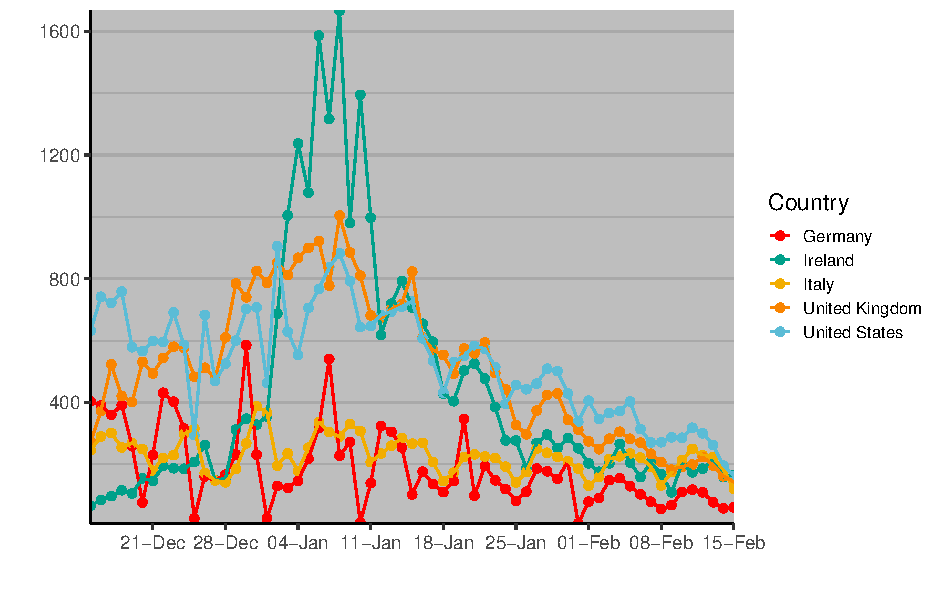
\includegraphics[width=0.9\textwidth]{compare-all.pdf}
\endminipage
\caption{Comparison of Ireland with various countries, daily cases per million of the population}
\end{figure}




\subsection{Previous work on Covid-19 identification and modeling}
Research in the area of modeling the spread of the pandemic has been extensive and as such it would be impossible to acknowledge all the previous and ongoing work here. I would like to note a few studies (first published towards the beginning of the pandemic) that differ to my approach.

The work involving \textit{external} factors such as government travel restrictions or full lockdowns, carried out by \cite{flaxman20}, was widely read. However, it was also criticised for their model (which tried to assign a quantitative effect of interventions on disease spread for multiple countries) lacking practical statistical distinguishability, and prompted revisions.

Artificial intelligence models have also been employed to track disease outbreaks in more local areas. The model developed by \cite{SrinivasaRao2020}, which relies on phone–based surveys, certainly has the long-run potential to keep the public informed and hopefully reduce the the severity of outbreaks in areas where the app is widely used. One drawback of the initial model was its estimation of the peak of case numbers (which is notoriously difficult to predict) being the highest value in the case numbers so far.This does not take into account the shape of many time series during the early stages of the virus outbreak. For example, a strictly increasing time series would have its maximum at the latest time.


\subsection{Key aims}

This project is based on the work in \cite{grigor20}, where I attempt to reconstruct the recurrence relation to model the pandemic. This is a largely mathematical model (based on practical assumptions), but of course does not fit well in the long run. It is efficient at explaining singular phases of the pandemic (with a consistent trend), and calculating the infamous $R_0$ number, defined below, from \cite{epid08}. 

\begin{ndefinition} 
The number $R_0$ is called
the \textit{basic reproduction number} and is unquestionably the most important quantity to consider when analyzing any epidemic model for an infectious disease. Each infective individual can be expected to infect $R_0$ individuals. 
\end{ndefinition}

\subsection{Limitations}
There are some limitations to the models used in this paper, some of which we can quickl see after the visualisation of the models versus actual cases reported:
\begin{itemize}
\item The models seem to fit well when there is an obvious trend in one direction. They do not perform well at or past a peak in case numbers. 
\item Countries may see their testing capabilies strained or varied, and so some reported numbers may be attributed to a later date than usual.
\item Vaccinations began in late 2020 to early 2021 and will likely affect the spread of the virus
\item The modeling is done on a univariate time series, whereas external facors such as population densities and other demographics. Spatial data would then be needed to model the disease spread, but this is beyond the scope ofthe paper.
\end{itemize}